\section{Evaluation}
\label{sec:evaluation}
% comment by Daniel: This section could be used to provide information on the methodology, general issues, selection process of the upcoming issues (sub sections) or similar...

In this section, we will first provide an evaluation of the AR game play components.
% TODO write about what we do secondly.

% AR-Komponente (Bewegung des Dämons, Werden die PoI’s wiedergefunden, etc.)
% - biggest challenge: ensuring that tracking points at PoI remain consistent as user approaches; old visual context is lost as they focus e.g. on a single part of the desktop --> might cause ARCore to recalc coordinate system (could have been nice to pause allocation of tracking points and rely on accelerometer, but ARCore does not support this)
\subsection{Tracking Point Accuracy}
The most important limitation for the augmented reality subsystem we encountered was the stability of tracking points in the virtual space.
As described before, quick movement caused ARCore to lose track of many of the points and creating new ones, thus invalidating potentially crucial information about the room.
Since the setting of the game encourages the feeling of hunting after the demon, quick movements are unfortunately an expected and potentially necessary part of the game.
Further problems arose when the user moved closer towards a point of interest at which the demon was sitting.
As they approach the point, a lot of points all around the room will "disappear" as the frame of the camera narrows in on the area of interest.
This would not necessarily be a problem, however ARCore will constantly recompute the coordinate system and make considerable corrections to the origin when it loses important tracking information or gets a lot of new points in an area.
Often, this had the effect of the demon getting farther and farther away from the player as they approach it, even though it appeared to be sitting at a constant position.

At the time of writing, ARCore does not expose an option to \enquote{freeze} the coordinate system.
This functionality would have likely remedied our issues, if we froze the coordinate system when switching to the capturing phase, where stable positions are essential, and relied on the phone's accelerometer and picture data to move the camera in the existing virtual space.
ARCore did not expose sufficient access to the lower level system for us to try this approach by ourselves, so we will either have to wait for its developers to add this functionality or use and modify an open source augmented reality framework to solve this specific use case.

% FIXME: to be tested further:
% - by defining anchors on the relevant tracking points, ARCore will ensure most of the time that objects remain within reach -- timeout and fallback to showing spell even though user is not close enough otherwise
As a workaround to this issue, we make use of the ARCore anchors, which will update and move around the coordinate system to try and make up for changes to the coordinate system's origin or scale.
This helped most of the time to ensure that the demon will at least be within the activation distance for the capturing phase, but it still appeared to coast around the spot.
To not block the game altogether when the demon attaches to a point with incorrect depth, making it impossible for to the user to come close enough, we added a timeout that will move the game onwards in the hope that the next point may be better.

\subsection{Demon Movement}

% Comment from daniel: I would like to see lots of images here, e.g., show a stupid positioning due to errors, or how does good tracking accuracy compare to a bad one by example
\begin{figure}
    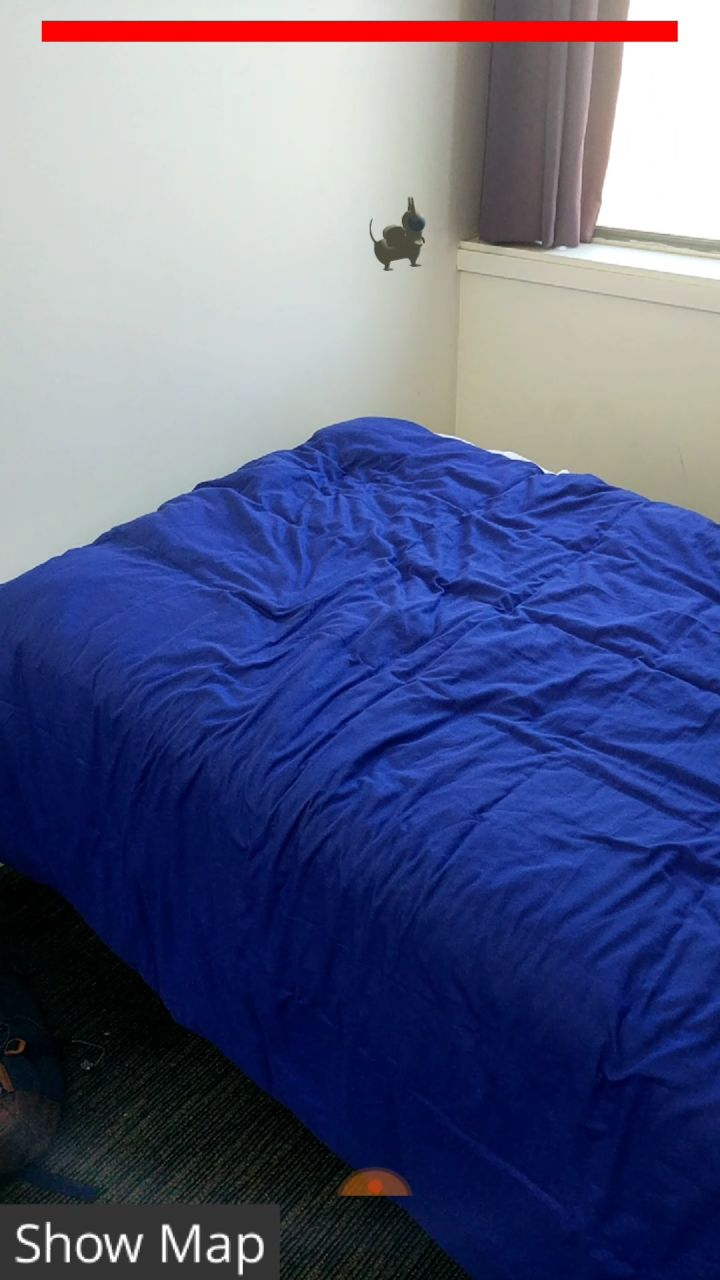
\includegraphics[height=8cm]{graphics/demon-wrong-depth.jpg}
    \caption{The demon appears to be floating inside the wall. The debug output in the console reported a distance from the camera of about 7 meters while this frame was captured. The distance from the camera to the wall is about 2 meters.}
    \label{fig:demon_wrong_depth}
\end{figure}

% - movement of demon feels weird at start, as dimensions of room are unknown
The movement of the demon in our current implementation is simplistic and makes next to no use of advanced possibilities, like collision detection.
This is mainly because the quality of the tracking points even for our room size estimation may vary greatly, so that we chose to use the simplest possible primitive volume in 3D space to reduce the chance of the demon getting locked within non-existing obstacles that have been formed by errors in the tracking point estimation.

% - placement of waypoints close to user confuse, but as they traverse the room and turn frequently it's hard to predict where they will be
Our concept of exploring the room size by encouraging the user to turn frequently at the start of the session, by making the room very small, may lead to some confusion as the demon appears to travel through impossible ways, for example through the user.
As the room quickly grows bigger, this may not be as much of an issue, however it may make sense to add a better waypoint system than simply selecting random points in the known space.
This may also help to make the demon feel like a more believable creature.

\subsection{User Experience}
% FIXME: to be evaluated if that applies to anyone else but me:
- handling of phone is tricky: most users held phone in right hand, shot w/ left hand in scanning phase. switch hands when entering capturing phase for drawing spells --> messes up coordinate system as phone points to floor temporarily

% Erkennung der Points of Interest
- Blurriness: Laplacian is not too precise, e.g. when using shallow focus, some regions are completely focused whereas some are totally blurry
--> will result in low blurriness value

% Brand-Detection

% Textanalyse mit OCR
- Wo wird im Bild Text erkannt?
- Kann dieser Text interpretiert werden, wenn ja, wie gut?
- Was sind Probleme? (Schriftart, Blurriness, distortion)

% Scalability
